\documentclass[conference]{IEEEtran}
\IEEEoverridecommandlockouts
% The preceding line is only needed to identify funding in the first footnote. If that is unneeded, please comment it out.
\usepackage{cite}
\usepackage{amsmath,amssymb,amsfonts}
\usepackage{algorithmic}
\usepackage{graphicx}
\usepackage{textcomp}
\usepackage{xcolor}
\usepackage{hyperref}
\hypersetup{
    colorlinks=true,
    linkcolor=blue,
    filecolor=magenta,      
    urlcolor=blue,
    pdftitle={Overleaf Example},
    pdfpagemode=FullScreen,
    }
\def\BibTeX{{\rm B\kern-.05em{\sc i\kern-.025em b}\kern-.08em
    T\kern-.1667em\lower.7ex\hbox{E}\kern-.125emX}}
\begin{document}

\title{Solutions for decentralized AI\\
}

\author{\IEEEauthorblockN{Sergi Hernández Burbano de Lara}
\IEEEauthorblockA{\textit{Data science student} \\
\textit{Universitat Pompeu Fabra}\\
Barcelona, Spain \\
sergi.hernandez01@estudiant.upf.edu}
\and
\IEEEauthorblockN{Sergi Vila Oriol}
\IEEEauthorblockA{\textit{Telecommunications student} \\
\textit{Universitat Pompeu Fabra}\\
Barcelona, Spain \\
sergi.vila02@estudiant.upf.edu}
\and
\IEEEauthorblockN{Edgar Espinós Murria}
\IEEEauthorblockA{\textit{Telecommunications student} \\
\textit{Universitat Pompeu Fabra}\\
Barcelona, Spain \\
edgar.espinos01@estudiant.upf.edu}
}
\maketitle

\begin{abstract}
As of 2023, Artificial Intelligence (AI) models are being developed, trained, and deployed by private companies in a centralized way. In a world where AI is going to be an important source of power, it is vital to find ways to decentralize this power.

In this paper, we explore solutions to decentralize AI models using Blockchain technologies so that anyone could afford to train an AI model and so that anyone could own a stake in them if they wish. We propose a consensus protocol that uses Deep Learning model training as Proof of Useful Work and a solution with Smart Contracts in Ethereum. We finally study their weaknesses and costs and propose an alternative solution using Layer-2 applications.
\end{abstract}

\begin{IEEEkeywords}
deep learning, blockchain, consensus protocol, smart contract, decentralized AI model
\end{IEEEkeywords}

\section{Introduction}
In recent years, the rapid advancements in Deep Learning have demonstrated the potential of AI models across various applications: from chatbots to image generators and beyond.

However, these technologies are usually owned and developed by companies that take on the role of designing the models and the algorithms, gathering data, and training the models with their own computing resources. In the future, it will be no surprise to also see governments taking a leading role in the development and use of Deep Learning technologies.

With these two scenarios in mind, it is natural to fear the power that companies and governments can accumulate against citizens by owning these models. Many experts from diverse fields such as philosophy, journalism, anthropology, law, and economics have already highlighted the risks associated with a highly centralized and monopolistic tech industry, including increased economic inequality and the potential for more authoritarian governments  \cite{b1} \cite{b2} \cite{b3} \cite{b4}.

Fortunately, alongside these developments, another technology that seeks decentralization has been emerging: Blockchain. This technology started as a decentralized network of computers that maintained an append-only immutable ledger of transactions \cite{b6} but has developed into a wider concept allowing even other kinds of decentralized applications.

In this paper, we ask ourselves if the centralization of the AI industry can be mitigated through the convergence of Blockchain and Deep Learning.

In particular, we would like a system where a developer designs a Deep Learning model and submits it for training at a negligible economical cost. The providers of computational power and data could be compensated for their work with an economic good in the form of a crypto-token that could be exchanged by other crypto-assets or could give the owner the right of making queries to the trained AI model.

\section{Our contribution}
First, we propose a consensus protocol that uses Deep Learning training as Proof of Useful Work. We present an impossibility result that demonstrates the practical challenges associated with such a protocol under our desired assumptions and properties.

We provide an alternative solution using smart contracts to train models and provide token-based incentives to the trainers and the data providers. Through empirical analysis, we demonstrate that this solution incurs significant costs in terms of gas.

Finally, we pose Layer-2 applications as a more realistic and scalable alternative to the decentralization of AI models.

By presenting these contributions, our research provides valuable insights into the challenges and potential solutions for decentralizing AI models, paving the way for future research about more democratized and inclusive AI ecosystems.

\section{Background, terminology and definitions}
\subsection{Blockchain background}
Blockchains address the State Machine Replication (SMR) problem, where multiple nodes aim to reach consensus on the true state of a system (whether it is a set of transactions, balances, variable values, or, related to this paper, the most optimal parameters of a Deep Learning model), even in the presence of Byzantine nodes.

Consensus protocols in that use Proof of Work revolve around the idea of miners competing to solve a problem that is hard to solve but easy to verify. Bitcoin's PoW uses the problem of breaking SHA-256 hashes as the problem that miners have to solve in order to be the leaders of a round.

This method successfully achieves the goal of randomly selecting a miner according to its share of computational power in a permissionless network.

Smart Contracts are another significant concept in the world of Blockchains. Smart Contracts are code deployed in the Blockchain that can be executed by anyone. Thanks to them being in the Blockchain, no one can restrict access to their functions and no one can manipulate its output.

\subsection{Deep Learning background}
Deep Learning is a type of machine learning based on artificial neural networks in which multiple layers of processing are used to extract progressively higher-level features from data to learn patterns (definition from Oxford Languages).

We use the term Deep Learning model to refer to a certain Deep Learning architecture with trainable parameters $W$ that are initialized randomly and trained iteratively using some optimization algorithm like stochastic gradient descent.

A model can be as simple as a linear regression with 2 parameters (the bias $w_0$ and the slope of the line $w_1$) or more complex like GPT-2, which has over 1.5B parameters\cite{b5}.

The training of the model depends on the choice of some hyperparameters. These hyperparameters include the learning rate $\alpha$, the optimization algorithm, or the number and size of layers in the neural network. These can influence both the results and the duration of the training process.

So training Deep Learning models is a game of finding the optimal parameters thanks to optimization algorithms, and finding the optimal hyperparameters through a process that involves part trial and error and part educated guesses. Moreover, even if there are algorithms that can find local minima like gradient descent, algorithms that find global optimum are unknown yet.

\section{Embedding decentralized AI in the consensus protocol}
\subsection{Previous work}
Several attempts have been made to develop Proof of Useful Work protocols that leverage Deep Learning training as the computationally intensive task for miners:

\begin{itemize}
\item In Proof-of-Learning (2019) \cite{b7}, the authors propose a consensus protocol where ``Suppliers" publish machine learning tasks that are solved by ``Trainers". The solutions provided by ``Trainers" are evaluated by ``Validators" that choose the winning node and add the next block to the Blockchain. An unaddressed issue in this paper is how to avoid ``Trainers" to simultaneously act as ``Validators" and rank their own solutions as the best.
\item The authors of Coin.AI (2019) \cite{b8} propose using the hash of the previous blocks to determine the hyperparameters used by miners to train the models to ensure the immutability of the Blockchain. They also propose a Proof of Storage distributed system to incentivize nodes to store the models after training. The winner is the first miner that achieves a certain quality threshold. So there is no ``Validator" ranking the solutions.
\item BlockML (2019) \cite{b9} also proposes having ``Supplier" and ``Miner" roles. In this case, miners themselves collectively rank the solutions proposed by other miners, but the authors do not provide a solution to prevent ``Miners" from stealing each other solutions. They split each round into a training phase and an evaluation phase.
\item In Proof-of-Deep-Learning (2019) \cite{b10}, they only allow one problem submitter that should be honest (they call it ``model requester"). They also split each round into two phases: the first in which miners train the model and commit to it by publishing it on the Blockchain, and a second phase in which they reveal it to other nodes for them to rank them and choose a winner.
\item The Proof of Artificial Intelligence (PAI) (2020) \cite{b11} network is composed of many entities: problem submitters (called "Clients"), "Miners" that perform the training, "Supervisors", "Evaluators" that evaluate the trained models, and "Verifiers". In this case, each round is splitted in four: registration, initialization, training and finalization.
\item More recent work such as DLBC (2020)\cite{b12}, Proof of Learning (PoLe) (2020)\cite{b13}, or CrowdMine (2022)\cite{b14} propose very similar protocols to the ones explained before.

\end{itemize}

As the authors of BlockML cleverly point out, using randomly generated Deep Learning problems is not useful by construction. So we need to introduce a new entity to the game: problem suppliers.

Except for Proof-of-Deep-Learning (2019), where they assumed a single supplier that should be honest, all the other suggested protocols require problem suppliers to provide a reward for the winning miner. The authors of CrowdMine even propose burning part of the rewards instead of giving them in full to the winner to compensate from MEV incentives.

We ask ourselves if this is a necessary requirement to avoid attacks from dishonest suppliers.

\subsection{Impossibility proof sketch}

Let $\Pi$ be a consensus protocol under the permissionless setting assumption in which the leader of each round wins a fixed newly-minted reward and is selected as the node with higher performance in solving a user-proposed problem (like optimizing a deep learning model), such that these problems are submitted for free by non-authenticated users to a pool of problems and attempted to be solved by miners.

Theorem: such a protocol cannot exist without preventing Byzantine nodes from gaining rewards with a higher probability than honest nodes, even with $f=1$.

Let a network have 3 nodes where 2 nodes are honest and run $\Pi$, and the other node is Byzantine.

If all nodes were honest, at round $t$, they would try to solve the $t$'th problem. Each node would solve it with random degrees of success, making the choice of the leader of the round effectively random.

But, since nodes and users are anonymous and unauthenticated, a player can be both a node and a user. Thus, the Byzantine player can submit to the pool a hard problem for which he already knows the solution. When the problem gets to be solved by all the nodes, the Byzantine node can provide the most optimal answer to the problem with higher probability than the other nodes because he had prior knowledge of the problem. So dishonest nodes can manipulate their probability of being chosen as the leaders.

We arrive at a contradiction, so we conclude that a protocol like $\Pi$ cannot exist without preventing nodes from manipulating their probability of winning rewards. 

At the same time, since problems are submitted at zero cost to the pool, players are not disincentivized to spam the pool with problems in which they have no real interest.

\subsection{Protocol sketch}

We have implemented our own functional Deep Learning consensus protocol so that in the next section we are able to do simulations in Python.

The protocol we implemented was based on some ideas from previously published protocols and other ideas of our own. It is designed to be easy to implement and simple to understand. Its correctness and safety are still to be studied.

It has two possible entities:

\begin{itemize}
\item ``submitters'' that wish to outsource the work of discovering a model $f$ that maps some input distribution $X$ to an output distribution $Y$ with the maximum accuracy possible;
\item and ``miners'' that are willing to find that model $f$, which depends on parameters $W$ and other hyperparameters.
\end{itemize} 
Miners try to solve the same problem all at the same time. We assume there is a method for all the miners to agree on the order of the submitters (it could be in a FIFO order, or by the amount of rewards they provide if any).

The protocol runs for sequential rounds at the end of which all honest nodes should agree on one block to be appended to their local histories. Each round has three phases:
\begin{enumerate}
    \item ``Training phase'', in which:
    \begin{enumerate}
        \item the submitter broadcasts a training dataset $\{\mathcal X_\text{train},\mathcal Y_\text{train}\}$ to all miners;
        \item miners train their models $\{f,W\}^{(i)}$ using the training data, where $i$ denotes the $i$'th miner;
        \item miners have to commit to their final model $\{f,W\}^{(i)}$ by sending a hash $h^{(i)}$ of it to the submitter before a timeout.
    \end{enumerate}
    \item ``Evaluation phase'', in which:
    \begin{enumerate}
        \item after the timeout, the submitter broadcasts the test input $\mathcal X_\text{test}$ to all miners;
        \item miners compute their estimates for the test output using their model $f^{(i)}(x_{\text{test}}|W^{(i)})=\hat y_{\text{test}}^{(i)}$;
        \item miners send their estimates $\hat{\mathcal Y}_{\text{test}}^{(i)}$ to the submitter (this serves as a Zero-Knowledge proof for the submitter that the miner has a way to predict $y$ from $x$ with some deterministic accuracy);
        \item the submitter computes the accuracy $a^{(i)}$ of the model of each miner $i$ by comparing their estimates $\hat{\mathcal Y}_{\text{test}}^{(i)}$ with the real test dataset $\mathcal Y_{\text{test}}$.
    \end{enumerate}
    \item ``Awarding phase'', in which:
    \begin{enumerate}
        \item the submitter ranks miners by their accuracy;
        \item the submitter sends a signed message to the miner with the most accuracy (denoted $w$) certifying it as the winner of the round;
        \item the submitter sends the hash $h^{(w)}$ of the model and the estimate $\hat{\mathcal Y}_{\text{test}}^{(w)}$ of the winner to all the miners;
        \item the winner is then allowed to build a block in which he will include the signed certificate of the submitter and the model $\{f,W\}^{(w)}$;
        \item the block is broadcasted to all other miners;
        \item miners verify the block by checking that:
        \begin{enumerate}
            \item it includes the certificate of the submitter of the round,
            \item the hash of the published model $\{f,W\}^{(w)}$ corresponds with the hash $h^{(w)}$ the winner committed to during the training phase,
            \item and that the published model $\{f,W\}^{(w)}$ indeed maps $\mathcal X_\text{test}$ to the estimate $\hat{\mathcal Y}_{\text{test}}^{(w)}$ to which the winner committed to during the evaluation phase.
        \end{enumerate}
        If the published model does not correspond with the hash or is not the model that the winner used to compute $\hat{\mathcal Y}_{\text{test}}^{(w)}$, honest nodes will not add the block to their local histories and will notify the misconduct to the submitter that will choose the next model with best accuracy and will start again from step 3b.
        
        If the model is correctly published, honest nodes add the block to their local history and a new round starts.
    \end{enumerate}
\end{enumerate}

This protocol certainly works assuming honest behavior from all players and is designed to be resistant to some attacks. Nonetheless, by now, it is just designed for testing purposes.

With the definition above, the protocol does not force submitters to pay a fee or provide a reward. Even if we already proved that it was necessary, we will assume it is not and test the assumption with an experiment in the following section.

Future work could include studying the correctness and security of this protocol if submitters were required to provide rewards, and comparing it with previously proposed protocols.

\subsection{Experiment in Python}
After implementing the aforementioned protocol, we simulate a network of nodes running the protocol where one of them is Byzantine and executes the attack discussed before: performing the submitter and miner roles simultaneously and submitting pre-solved problems to the pool in order to gain the newly-minted rewards with higher probability than the honest nodes.

As we can see in Figure 1, if all five nodes are honest and have the same computational power, the share of rewards after 1000 rounds is equally split among them ($\approx20\%$ each).

\begin{figure}[htbp]
\centerline{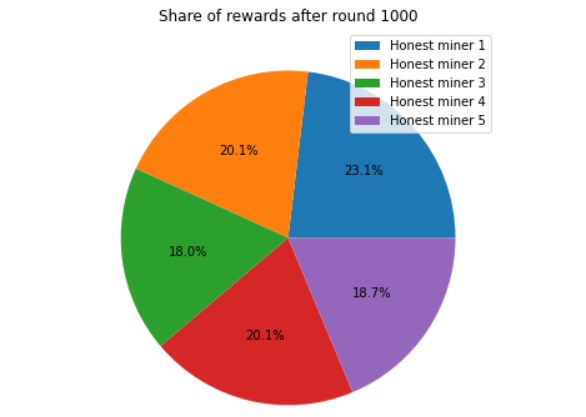
\includegraphics[scale=0.50]{share-rewards-all-honest.png}}
\caption{Share of rewards after round 1000 with all nodes being honest.}
\label{fig}
\end{figure}

On the other hand, as we see in Figure 2, with one Byzantine node submitting pre-solved problems, the dishonest player earns more rewards than the rest. In particular, in the simulation, the Byzantine node submitted $50\%$ of the problems of the pool, making him earn $50\%$ of the rewards plus $10\%$ that come from splitting the rewards of the other problems with the rest of miners equally.

\begin{figure}[htbp]
\centerline{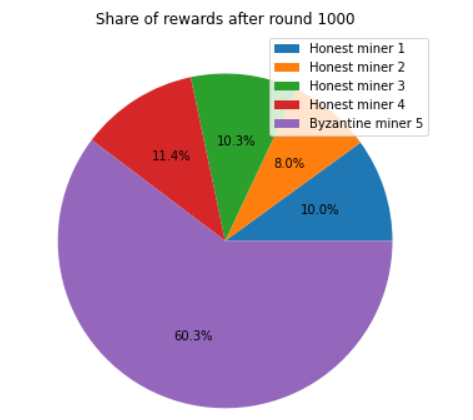
\includegraphics[scale=0.50]{share-rewards-one-dishonest.png}}
\caption{Share of rewards after round 1000 with one dishonest node.}
\label{fig}
\end{figure}

So, from the proof sketch and the experiment, we conclude that without rewards and/or fees provided by the submitters, miners can manipulate their probability of mining a block and thus win the newly-minted reward.

The simulation code can be found in GitHub: \url{https://github.com/SergiHernandez/DecentralizedAI}

\section{Implementing decentralized AI in smart contracts}

Having seen that it is impossible to have such a decentralized AI solution implemented in the consensus protocol of a Blockchain, we ask ourselves if it would be feasible to have it implemented in smart contracts.

\subsection{Previous work}

\begin{itemize}
\item Galaxy Learning (2019)\cite{b15} is the first attempt known to us to decentralize data storage and AI model training at the same time. They also propose incentives to data providers as a way for individuals to leverage their power against companies or institutions that regularly make use of their data. For the training mechanism, they suggest federated learning.
\item The Microsoft's SUM project (2019)\cite{b16} also proposes a smart-contract-based framework for sharing and improving machine learning models. They define a way to incentivize users to provide more training data and punish wrong data submissions.
\item In Incentivized Decentralized Machine Learning (2023)\cite{b17} and BRAIN (2023)\cite{b18}, the training is done by trainers off-chain and they then propose updates using a commit-reveal mechanism. The smart contract then scores and rewards the updates that are most optimal.
\end{itemize}

\subsection{Experiment in Solidity and Brownie}

To assess the feasibility of training a simple model like a linear regression model within a smart contract, we conducted a test.

The test involved storing the training data in the smart contract using two arrays, namely, $x$ and $y$. Additionally, we implemented a function called "train()" within the smart contract that utilizes stochastic gradient descent to update the parameter values $w_0$ and $w_1$.

We then deployed the Solidity smart contract using the Brownie framework and used the web3 library to approximate gas costs.

The Solidity smart contract code can be found in GitHub: \url{https://github.com/SergiHernandez/DecentralizedAI}

\subsection{Gas cost analysis}

Using the web3 library, we can approximate the gas costs of executing the linear regression smart contract.

\begin{table}[htbp]
\caption{Gas costs of on-chain linear regression$^{\mathrm{a}}$}
\begin{center}
\begin{tabular}{|c|c|c|c|}

\hline
\textbf{Action}&\textbf{Gas cost}&\textbf{Gwei cost}&\textbf{in USD} \\

\hline
addData()& 103,299 & 2,065,980 & $\$3.59$  \\ \hline
train()& 138,433 & 2,768,660 & $\$4.82$ \\  \hline
Full test execution& 276,305,223 & 5,526,104,460 & $\$9,626.47$\\
\hline
\multicolumn{4}{c} \text{$^{\mathrm{a}}$With 1 gas $\approx$ 20 gwei and 1 ETH $\approx$ 1,742 USD as of June 2023}
\end{tabular}
\label{tab1}
\end{center}
\end{table}

As we see in Table 1, the cost of fitting a line to just nine data points in the Ethereum chain can amount to thousands of dollars. To put this into perspective, executing the same linear regression algorithm in Python on a low-cost laptop would only take a few seconds and consume minimal energy, amounting to just a few cents.

\section{Conclusions}

In this study, we explored the feasibility of implementing decentralized AI solutions within consensus protocols and smart contracts. We began by examining existing protocols and their limitations in achieving a fair and secure decentralized AI system. Through an impossibility proof, we demonstrated that it is impossible to prevent Byzantine nodes from manipulating their probability of winning rewards in a permissionless consensus protocol, even with a single Byzantine node. Additionally, we examined the possibility of implementing decentralized AI in smart contracts and evaluated the gas costs associated with executing a linear regression model. The gas costs on the Ethereum blockchain were found to be significantly higher compared to executing the same task on a traditional computing device.

Considering the limitations and challenges identified throughout our analysis, we conclude that achieving a fully decentralized and efficient AI system within consensus protocols and smart contracts remains a complex task. While previous works have proposed innovative solutions, such as federated learning and incentivization mechanisms, further research and development are required to address scalability, security, and cost-effectiveness concerns.

Therefore, our solutions are:
\begin{itemize}
\item Embedding decentralized AI in the consensus protocol but requiring submitters to provide rewards.
\item Using a smart contract approach but move to a Layer 2 setting that would allow greater scalability through the reduction of gas costs.
\end{itemize}

In conclusion, while the vision of decentralized AI holds great promise for democratizing access to AI technologies and enhancing privacy, achieving its full potential requires innovative solutions and a deep understanding of the unique challenges posed by decentralized systems.

\begin{thebibliography}{00}

\bibitem{b1} Peirano, M. (2019). El enemigo conoce el sistema / The Enemy Knows the System. DEBATE.

\bibitem{b2} The Economist. (2023, June 10). Yuval Noah Harari argues that AI has hacked the operating system of human civilisation. The Economist. https://www.economist.com/by-invitation/2023/04/28/yuval-noah-harari-argues-that-ai-has-hacked-the-operating-system-of-human-civilisation.

\bibitem{b3} euronews. (2019, May 14). A.I. is as threatening as climate change and nuclear war, says historian Yuval Noah Harari [Video]. https://www.euronews.com/2019/05/14/a-i-is-as-threatening-as-climate-change-and-nuclear-war-says-philosopher-yuval-noah-harari.

\bibitem{b4} Stoller, M., Miller, S., Teachout, Z. (2020, April 10). Addressing Facebook and Google’s harms through a regulated competition approach. American Economic Liberties Project. https://www.economicliberties.us/our-work/addressing-facebook-and-googles-harms-through-a-regulated-competition-approach/.

\bibitem{b5} Radford, A., Wu, J., Child, R., Luan, D., Amodei, D., \& Sutskever, I. (2019). Language models are unsupervised multitask learners. OpenAI. https://d4mucfpksywv.cloudfront.net/better-language-models/language-models.pdf.

\bibitem{b6} Nakamoto, S. (2008) Bitcoin: A Peer-to-Peer Electronic Cash System. https://bitcoin.org/bitcoin.pdf.

\bibitem{b7} Bravo-Marquez, F., Reeves, S., \& Ugarte, M. (2019). Proof-of-Learning: A Blockchain Consensus Mechanism Based on Machine Learning Competitions. https://doi.org/10.1109/dappcon.2019.00023.

\bibitem{b8} Baldominos, A., \& Saez, Y. (2019). Coin.AI: A Proof-of-Useful-Work Scheme for Blockchain-Based Distributed Deep Learning. Entropy, 21(8), 723. https://doi.org/10.3390/e21080723.

\bibitem{b9} Merlina, A. (2019). BlockML: A Useful Proof of Work System Based on Machine Learning Tasks. Association for Computing Machinery. https://doi.org/10.1145/3366624.3368156.

\bibitem{b10} C. Chenli, B. Li, Y. Shi \& T. Jung. (2019). Energy-recycling Blockchain with Proof-of-Deep-Learning. IEEE International Conference on Blockchain and Cryptocurrency (ICBC), pp. 19-23. https://doi.org/10.48550/arXiv.1902.03912.

\bibitem{b11} Lihu, A., Du, J., Barjaktarevic, I., Gerzanics, P., \& Harvilla, M. (2020). A Proof of Useful Work for Artificial Intelligence on the Blockchain. 
https://doi.org/10.48550/arXiv.2001.09244.

\bibitem{b12} Li, B., Chenli, C., Xu, X., Shi, Y., \& Jung, T. (2019). DLBC: A deep learning-based consensus in blockchains for deep learning services. 
https://doi.org/10.48550/arXiv.1904.07349.

\bibitem{b13} Lan, Y., Liu, Y., Li, B., \& Miao, C. (2021). Proof of Learning (PoLe): Empowering machine learning with consensus building on blockchains. In Proceedings of the AAAI Conference on Artificial Intelligence (Vol. 35, No. 18, pp. 16063-16066). 
https://doi.org/10.48550/arXiv.2007.15145.

\bibitem{b14} Chen, C., Cheng, Z., Qu, S., \& Fang, Z. (2022). Crowdsourcing Work as Mining: A Decentralized Computation and Storage Paradigm. 
https://doi.org/10.48550/arXiv.2211.06669.

\bibitem{b15} Wu, C., Xiao, J., Huang, G., \& Wu, F. (2019). Galaxy Learning - A Position Paper. 
https://doi.org/10.48550/arXiv.1905.00753

\bibitem{b16} Harris, J. D., \& Waggoner, B. (2019, July). Decentralized and collaborative AI on blockchain. In 2019 IEEE international conference on blockchain (Blockchain) (pp. 368-375). IEEE. https://doi.org/10.1109/Blockchain.2019.00057.

\bibitem{b17} Yu, H., Chen, H. Y., Lee, S., Vishwanath, S., Zheng, X., \& Julien, C. (2023). idml: Incentivized decentralized machine learning. 
https://doi.org/10.48550/arXiv.2304.05354

\bibitem{b18} Park, S., Lee, J., \& Moon, S. M. (2023). A Blockchain-based Platform for Reliable Inference and Training of Large-Scale Models. 
https://doi.org/10.48550/arXiv.2305.04062.

\end{thebibliography}
\end{document}